\begin{frame}{}

        \centering
        \begin{tikzpicture}
            \node (image) [anchor=south west, inner sep=0pt] {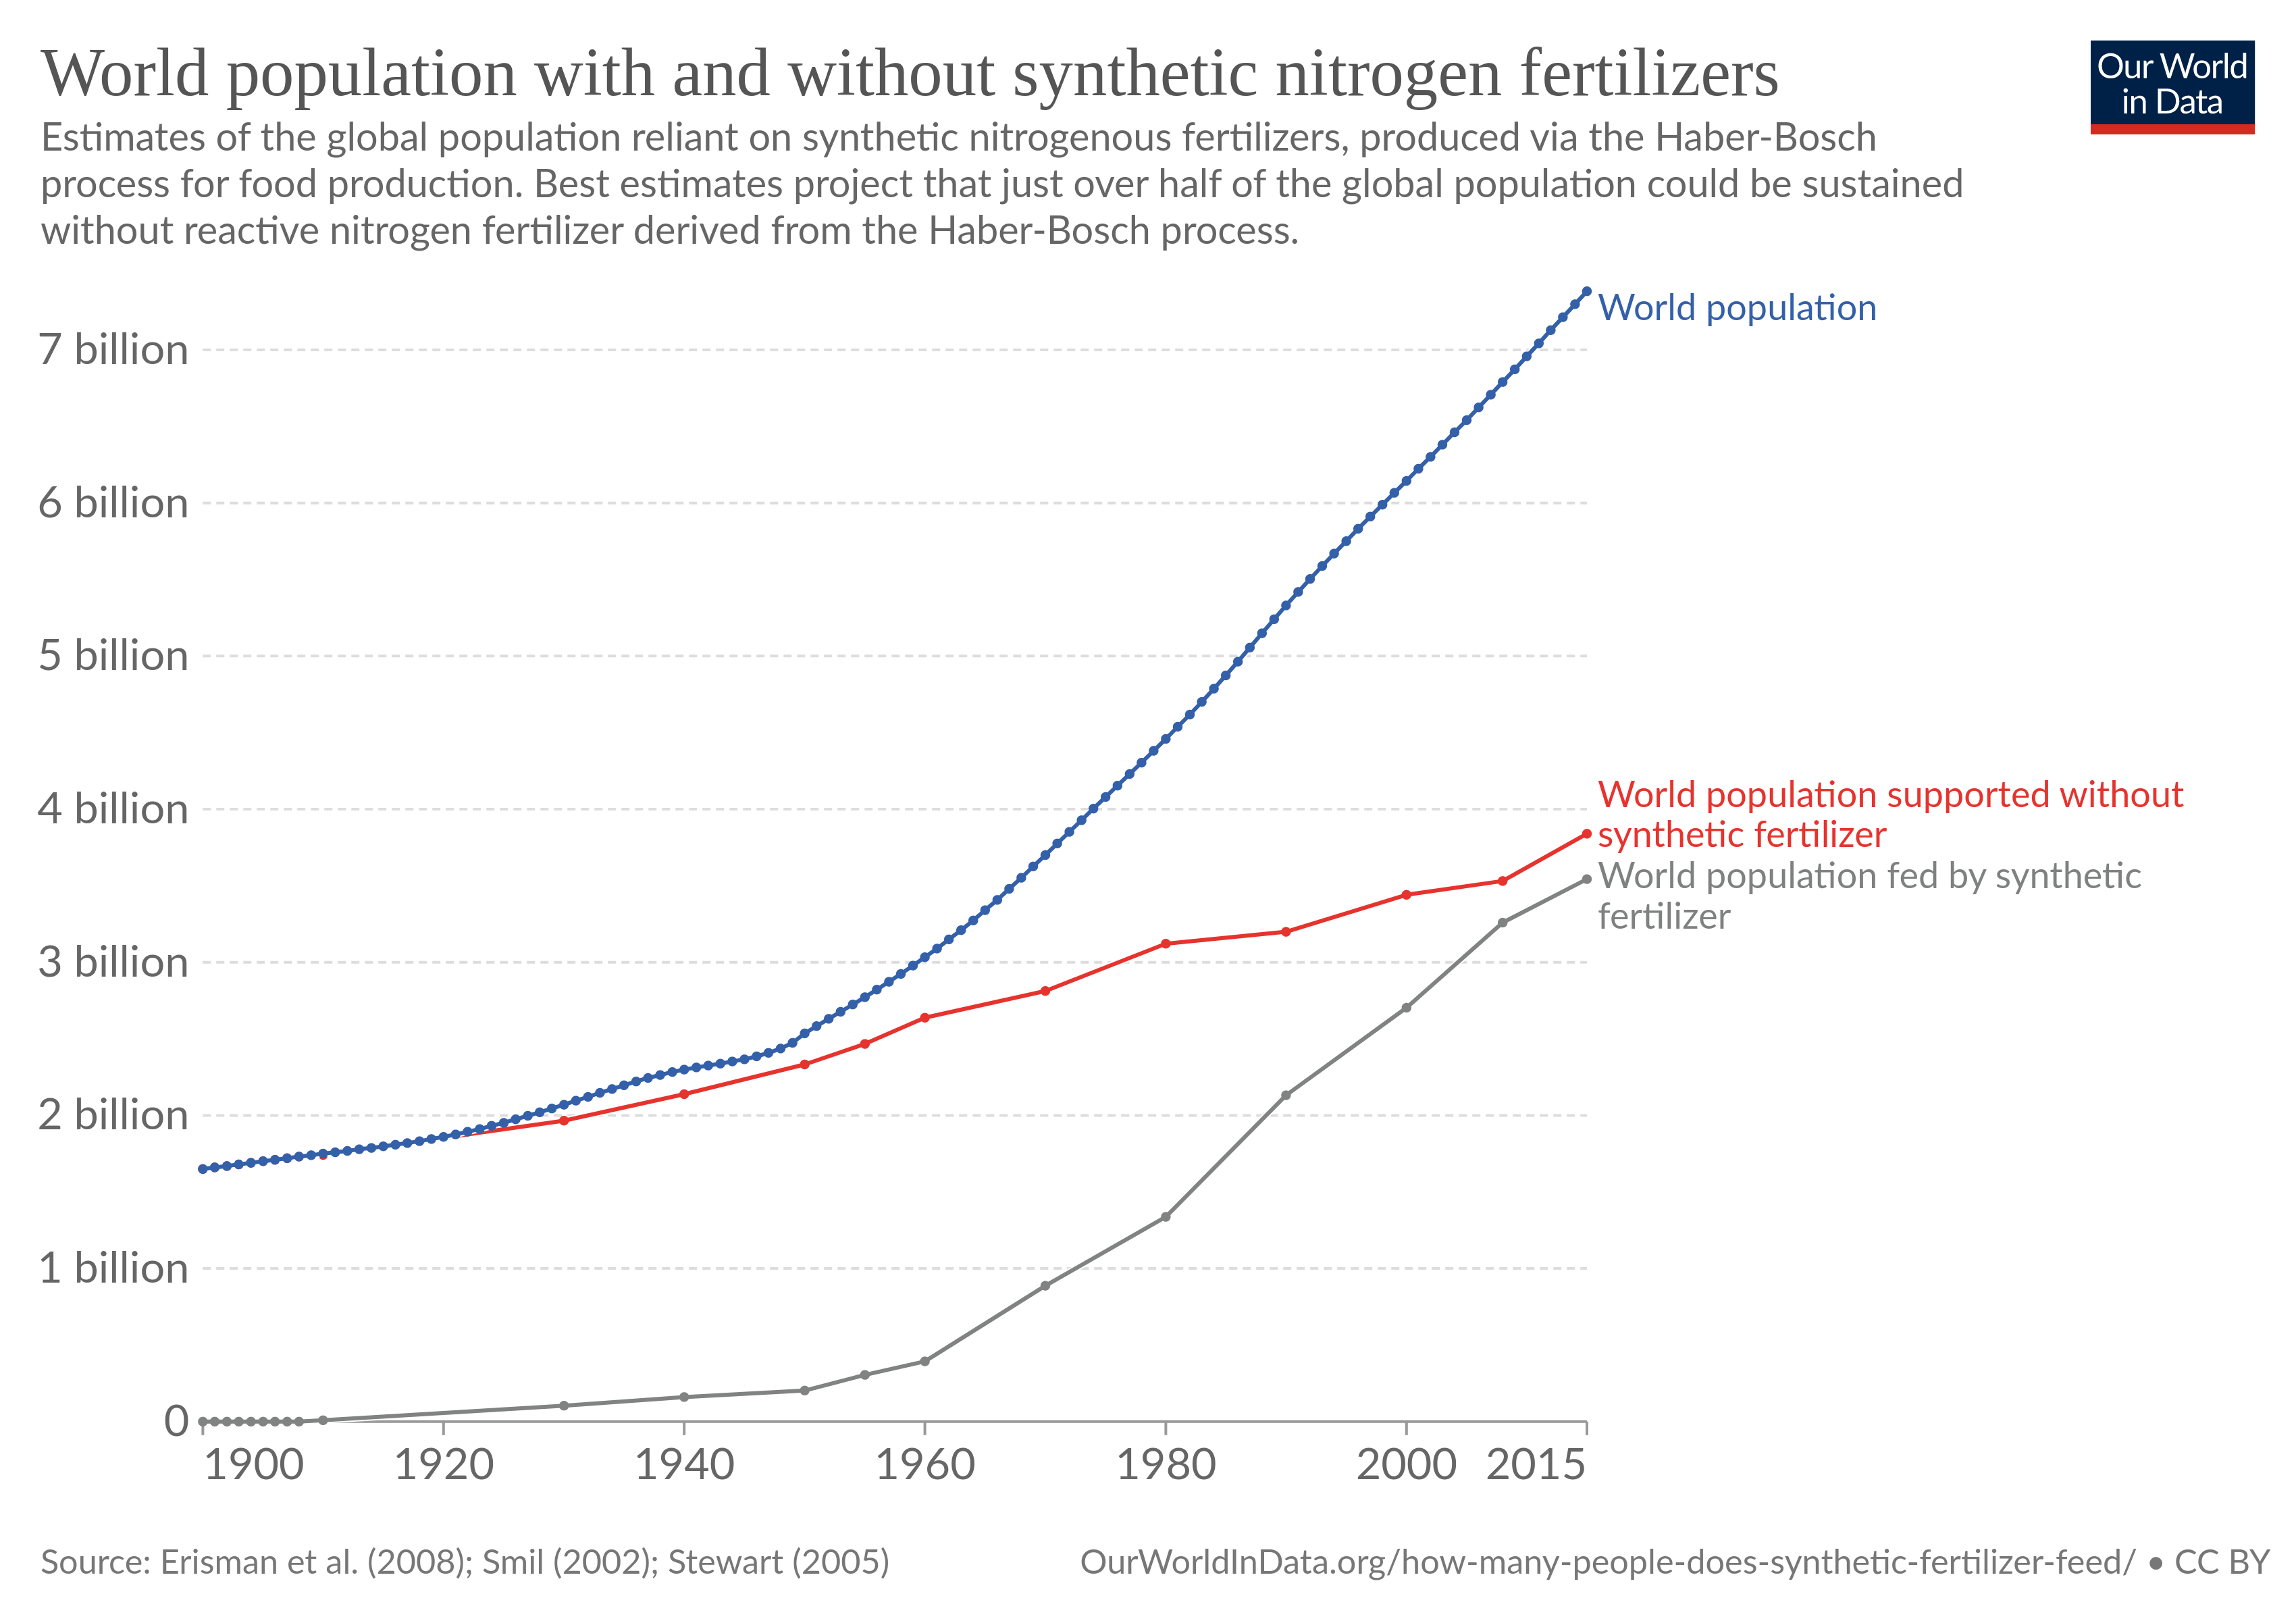
\includegraphics[width=0.99\textwidth]{Figures/worldindata/world-population-with-and-without-fertilizer.png}};
            \begin{scope}[x={(image.south east)}, y={(image.north west)}]
                \pause
                \node [text width=2.2cm,align=right] at (0.18, 0.7) (OP) {\textcolor{Ostwald}{Ostwald} process\\(1902)\\ \textrightarrow Nobel prize\\(1909)};
                \draw [-latex, ultra thick, Ostwald] (0.10,0.75) to (0.10,0.12);
                \pause
                \node [text width=2cm,align=right] at (0.19, 0.45) (HBP) {\textcolor{Haber}{Haber-Bosch}\\process (1908)\\ \textrightarrow Nobel prize\\(1918)};
                \draw [-latex, ultra thick, Haber] (0.13,0.4) to (0.13,0.12);
            \end{scope}
        \end{tikzpicture}
    
\end{frame}

